%!TEX root = ../../FYP_Dissertation.tex

When looking at the timing of individual tests of the MAD test suite we can see
that most of the instability comes from the Model Object tests. In Figure
\ref{fig:failed-test}, we can see a screenshot of three failed timing tests that
were calibrated to run in roughly 0.5 seconds and that for this run needed respectively
6, 4 and 68 seconds. We need then to investigate the reason for such results.

\begin{figure}[H]
    \centering
	\includegraphics[width=0.8\textwidth]{./Images/failed-test.png}
    \caption{Timing screenshot}
    \label{fig:failed-test}
\end{figure}

The Lua programming language doesn't actually have an object model but provide
mechanisms that allow anyone to build a custom object model fitting his needs.
Next section will present the one that as been built for MAD.

%===============================================================================
% Model object description
%===============================================================================

\section{Model object description}
\label{Sec:MO-descriptinon}

MAD object module implements the necessary machinery to support prototype-based
programming. When reading an attribute on an object, either the value is present
in the child object and it is returned or the query is passed to the parent
object recursively until the value is found or the original \emph{Object} is
reached. When a value is written the value is simply stored in the current
object (no lookups are performed). To understand how this object model is
implemented, a grasp of how lua handles tables and metatables is required.

To keep it simple here, lua tables are key-value stores that return \emph{nil} by
default if a key is not defined (see Section \ref{Subsec:table} for more).
Users have the possibility to associate a metatable to any tables. A metatable
is actually a standard lua table that contains special metamethods of which
the keys are defined by the lua language. The one that we are interested here is
the \emph{\_\_index} metamethod that defines how a table should react when accessing
an undefined key. If this is a method, the requested key is passed to this method
and it is executed, but if this \emph{\_\_index} contains another table, then this
table is queried instead of the first one. This is this mechanism that has been
used in MAD to implement the model object. Figure \ref{fig:MO-descriptinon} below
shows a schematic of the implementation of MAD object model.

\begin{figure}[H]
    \centering
    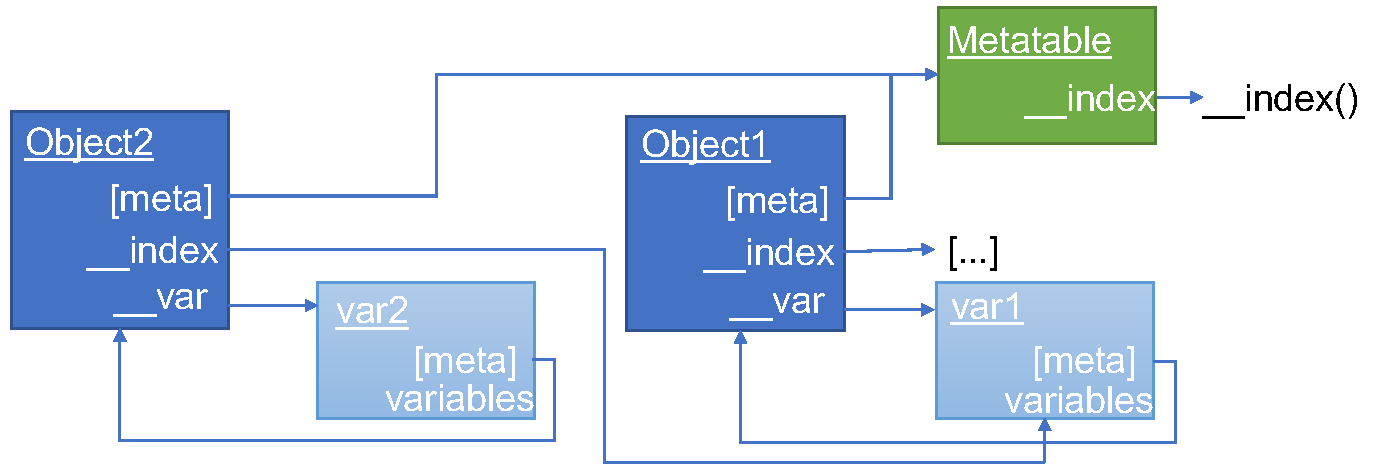
\includegraphics[width=\textwidth]{./Images/MO.pdf}
    \caption{Implementation of MAD object model}
    \label{fig:MO-descriptinon}
\end{figure}

On this figure, \emph{Object2} is the child of \emph{Object1}. To represent an
object, three lua tables are actually needed. The first one (in dark blue) is
the actual object passed around and manipulated by the user. It doesn't actually
contain any user data so when queried, the index function of its metatable (in
green) is executed instead. This metatable is by default the same for all objects
unless it is explicitly modified by the user. This index function gets the
\emph{var} table (in light blue) of the object and try to index it with the
requested key. If the key is defined, the corresponding value is returned,
otherwise the chaining lookup is triggered. Let's look at the example in the
figure when trying to query an undefined key in \emph{Object2}.
First the index function query \emph{var2} that doesn't contain it. Then, since
\emph{Object2} is the metatable of \emph{var2} (see the \emph{[meta]} arrow) and
the \emph{\_\_index} of \emph{Object2} links to \emph{var1}, \emph{var1} is queried.
This chaining is done recursively to the \emph{var} tables of its parents until the
key is found or the hierarchy entirely unrolled.

%===============================================================================
% Performance analysis
%===============================================================================

\section{Performance analysis}
\label{Sec:MO-perf-analys}

First of all, we are going to see how the JIT can make this object model
efficient and hoist away  all those costly lookups. In fact, the object model
described in the previous section might seem very slow as accessing variables
provided by a distant parent necessitates a big chain of lookups. In practice it
is not necessarily the case. Let's look at an example. Figure \ref{fig:MO-ex}
shows a model hierarchy that is transcribed in MAD by the lua code below from
lines 3 to 9. Since LuaJIT mainly compile loops, we are going to look at the IR
code (see Section \ref{Subsec:IR}) generated by LuaJIT for the loop lines 12 to 14
using the dump module (see Section \ref{Sec:Dump-mode}).

\begin{figure}[H]
    \centering
    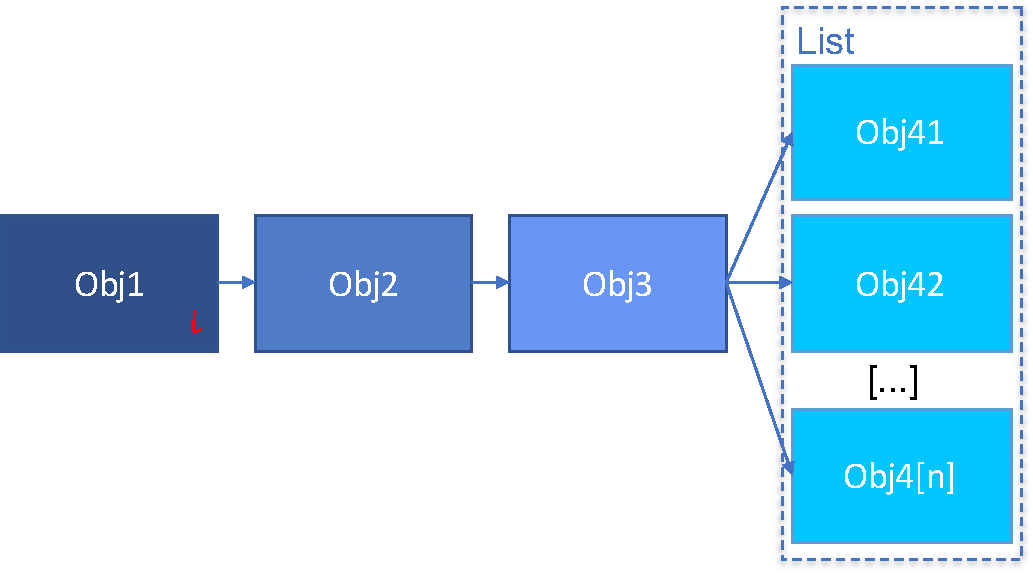
\includegraphics[width=0.8\textwidth]{./Images/MO-ex.pdf}
    \caption{Object inheritance of the example}
    \label{fig:MO-ex}
\end{figure}

\begin{lstlisting}[style=LuaStyle]
local object in MAD

-- object hierarchy
local obj1  = object "obj1"  { l = 42 }
local obj2  = obj1   "obj2"  { }
local obj3  = obj2   "obj3"  { }
local obj41 = obj3   "obj41" { }
local obj42 = obj3   "obj42" { }

-- loop
local sum = 0
for i=1,1e7 do
	sum = sum + obj41.l + obj42.l
end
\end{lstlisting}

\begin{figure}[H]
    \centering
    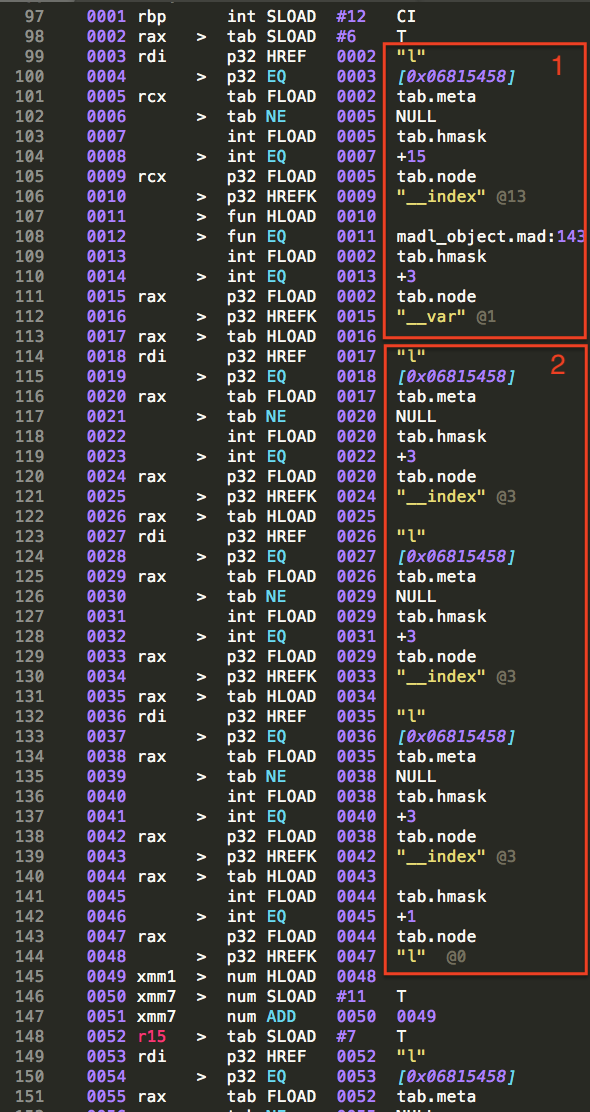
\includegraphics[height=13cm]{./Images/trace-1a}
    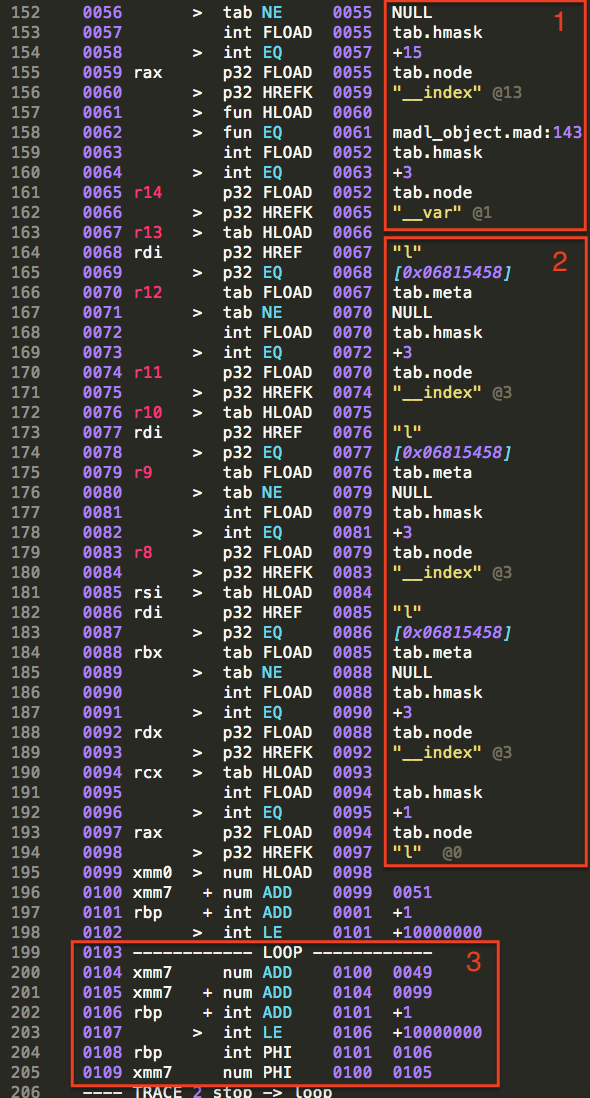
\includegraphics[height=13cm]{./Images/trace-1b}
    \caption{Screenshot of the example's loop trace}
    \label{fig:MO-ex-dump}
\end{figure}

Figure \ref{fig:MO-ex-dump} shows a screenshot of the dump trace. Without looking
at it too much in detail, we can see in the red squares labeled number one, the
access to the \emph{\_\_index} function that access the \emph{\_\_var} table to
query the "l" variable. Since this variable is not present in the first object
the hierarchy is unrolled three time (see the 3 "l" literals and the three
"\emph{\_\_index}" literals) in the red squares labeled with the number 2.
We have twice the same unrolling because the left screenshot shows the
unrolling for the first object (\emph{obj41}) and the right one shows the second
object (\emph{obj42}).

Now let's extract some general understanding from this example. Fist, the actual loop
is only the part in red labeled with the number three. We can see that it only
consists of the loop's counter and the additions. All other operations
from the model object has been successfully moved out of the loop making the loop
itself very small and efficient. This is the power of luaJIT. It can do that
using the loop optimization that consists of unrolling the loop once before the
actual loop itself executing all invariant operation and guards only once
(see \ref{Subsec:opt-loop} on loop optimization). Another thing to note here is
that the hierarchy chaining and the \emph{\_\_index} function is completely
inlined in the trace. This is always the case, there is never any explicit
control-flow possible in a trace with the exception of the actual LOOP currently
recorded, meaning that all functions and control-flow are inlined and specialized
to the runtime values.\\

Now let's look at another example based on the same hierarchy but slightly more
complex. Here the last level objects (\emph{obj4[n]}) are dynamic. Figure
\ref{fig:MO-ex-dump2} shows a screenshot of the dump trace for the second
example and we can clearly see that the hierarchy chaining is present both before
the loop (on the left) and inside the loop (on the right). This means that the
compiler hasn't been able to detect the invariance and produce a code similar to
the previous example, but it still manages to produce a single trace handling the
entire loop making it still performing better than with the VM interpreter.

\begin{lstlisting}[style=LuaStyle]
local object in MAD

-- object hierarchy
local obj1 = object "obj1" { l = 42 }
local obj2 = obj1   "obj2" { }
local obj3 = obj2   "obj3" { }

-- list of obj4[n]
local list = table.new(1e7, 0)
for i=1,1e7 do
	lists[i] = obj3 "obj4" {}
end

-- loop
local sum = 0
for i=1,1e7 do
	sum = sum + lists[i].l
end
\end{lstlisting}

\begin{figure}[H]
    \centering
    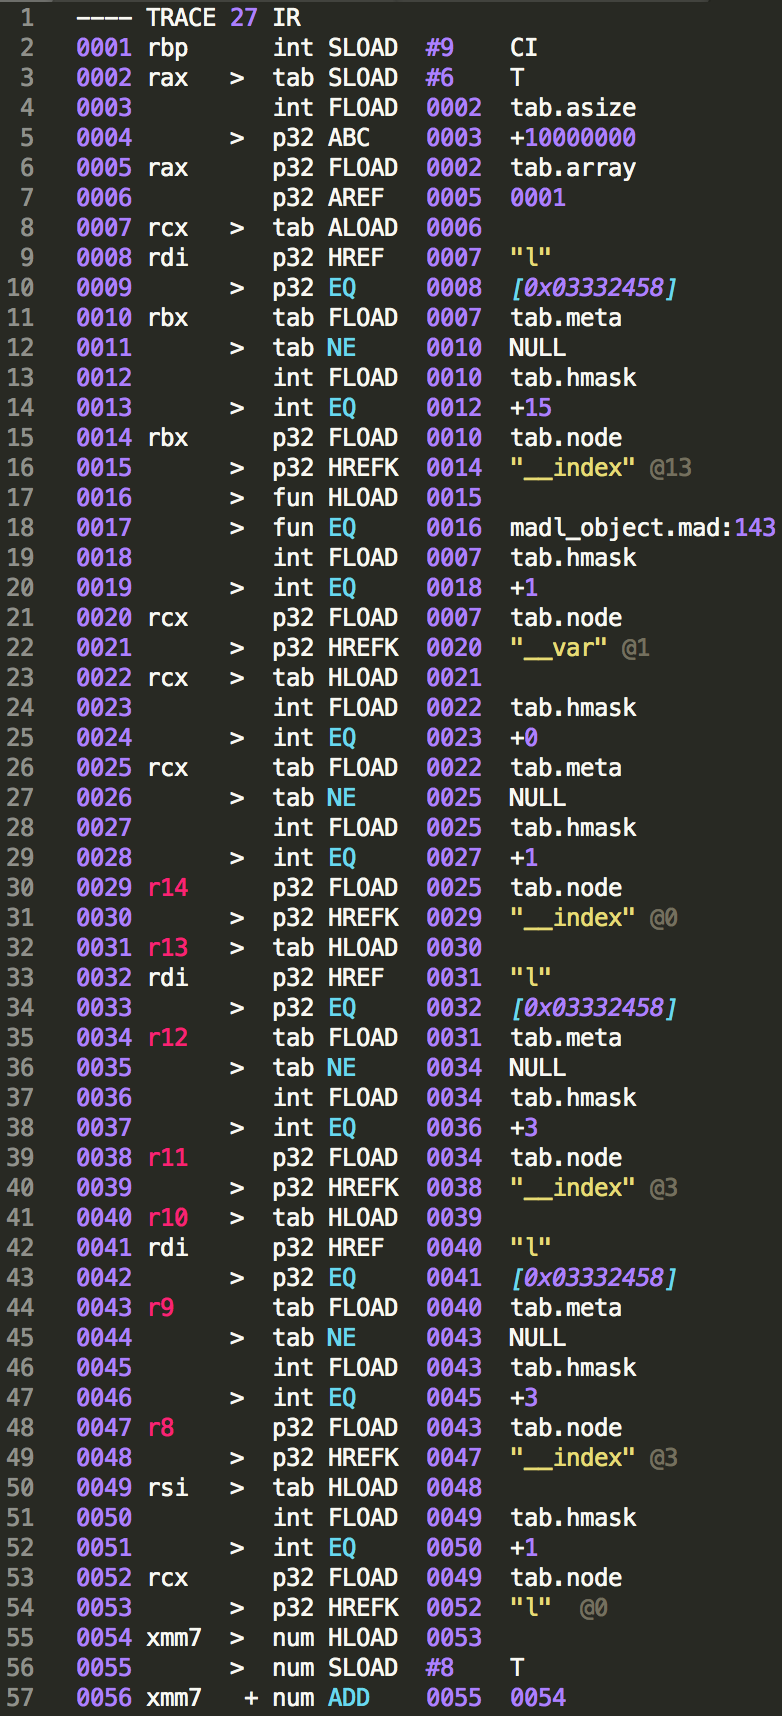
\includegraphics[height=13cm]{./Images/trace-2a}
    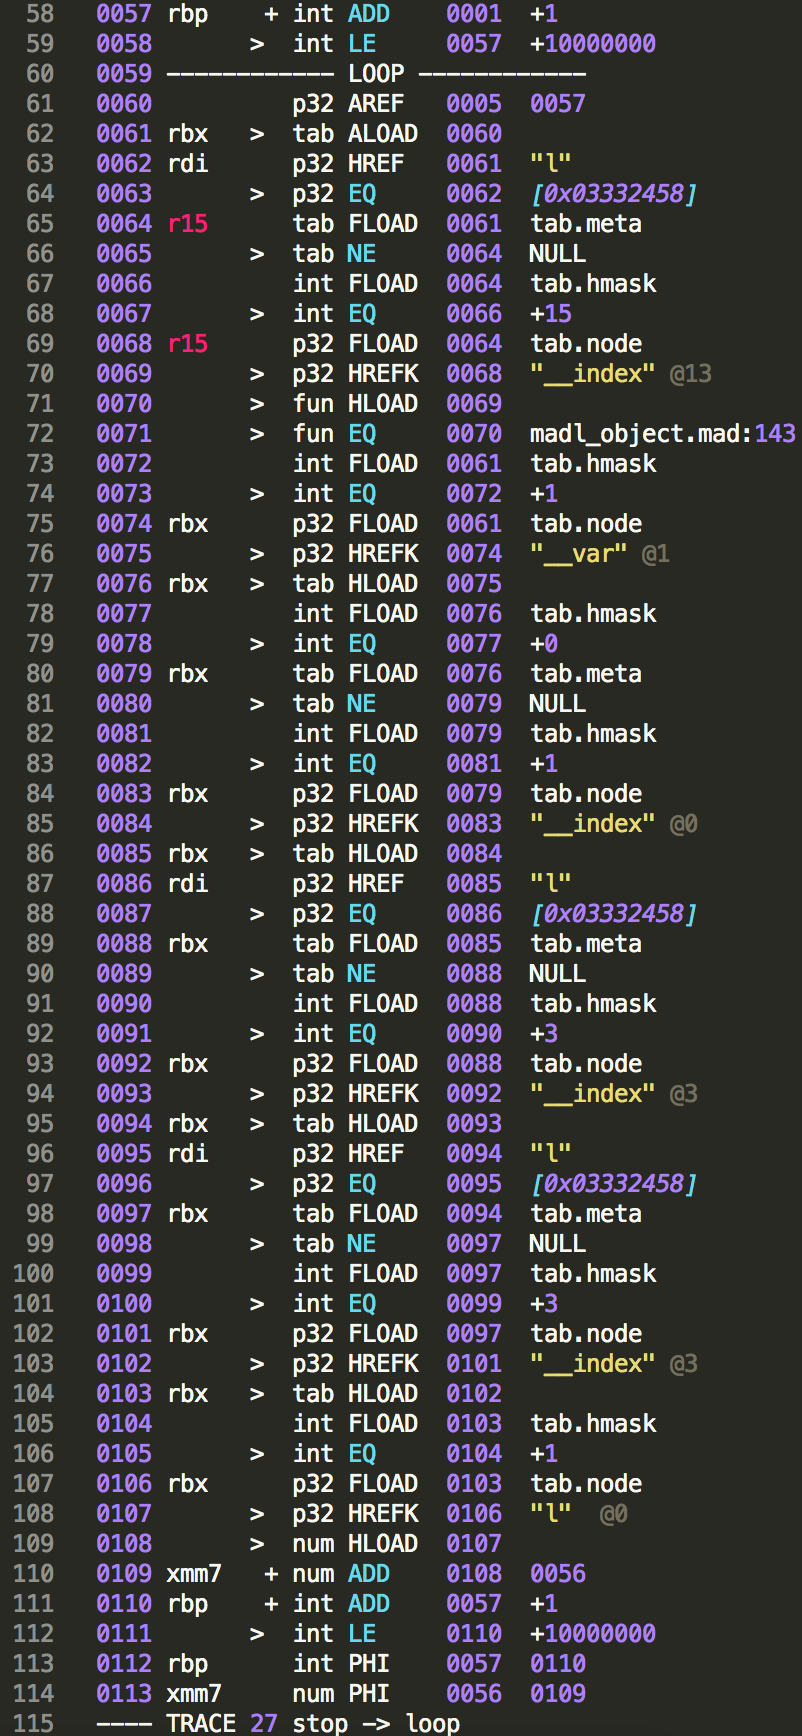
\includegraphics[height=13cm]{./Images/trace-2b}
    \caption{Screenshot of the second example's loop trace}
    \label{fig:MO-ex-dump2}
\end{figure}

%===============================================================================
% Instability possible explanation
%===============================================================================

\section{Possible explanations for performance hit}
\label{Sec:MO-insta}

The first thing interesting to note is that we can deactivate the JIT engine using
the \emph{-joff} command-line argument of LuaJIT and we can see that the VM is
slightly faster than the worst case scenario with the JIT activated. This can
be explained by the fact that in those cases the actual code is entirely run by
the VM, plus the compiler spent some time trying to record and generate traces
that end-up being aborted. Those claim can be verified by using the \emph{v}
option of the profiler (see Section \ref{Sec:Profiler}). The question now is :
why is it, that so much time is spent in the VM and why all those trace gets
aborted. This is where things gets complicated. When run stand-alone the
performance test mentioned earlier are always perfectly fine. It is depending of
the context, meaning the code that has been run before, that sometime makes those
test take a incredible amount of time. In addition of that the dump module of
LuaJIT is very useful when we want to study isolated problems but in this case
where the amount of code run influence the result, this tool generate to much
informations without much help to manipulate them, making it a needle in a
haystack kind of problem.\\

We will still present here some insight on this issue with some unsuccessful
tentative of solutions.

The first thing is that in some run the \emph{\_\_index}
function of the model object (presented in previous sections) gets blacklisted
(see Section \ref{Subsec:abort}). After that no hierarchy chaining can be
successfully recorded inside another trace making all of them running
exclusively in the VM. This is due to a mechanism of LuaJIT that we can call
\emph{cascading blacklisting} that consist of blacklisting bytecode that tries to
record a trace that hit another blacklisted bytecode. This is very inconvenient
because it means that a piece of code that can't be properly compiled for
whatever the reason can make the model object very slow for the rest of the run.
This is even more problematic knowing that blacklisting is permanent for the
lifetime of a particular bytecode, making it in this case for an entire run of
LuaJIT.

A second interesting fact to try to explain the instability part of the problem
is the fact that the hot path detection is very lazy and use the hashed program
counter (see Section \ref{Subsec:hot-path}) making false positive very easy to
occur. So any change to the code can change the bytecode alignment and the
potential false positive, changing in its turn the entire profile of the code
generated. This explanation is an educated guess and couldn't be formally proven
to be explaining in its own the change of behavior seen when slightly modifying
codes.

Another thing to consider is that in LuaJIT strings are internalized (see
Section \ref{Subsec:string-inter}) and that the memory address where they are
stored is used has "identifier" for string comparisons or hash-table placements.
Due to the ASLR (Address Space Layout Randomization) of many operating systems,
two consecutive runs of the exact same code will generate different address for
internalized string and possibly different placement inside hash-tables. In Lua
iterating over a hash-table can be done through the \emph{pairs} iterator that
doesn't enforce any special order (it just iterate sequentially over the internal
table structure), thus two runs can result in keys not being read in the same order,
making the JIT "see" the codes in a different order possibly changing false positive
and other behavior of the JIT.\\

Now let's have a look at a few modifications of LuaJIT that has been done to try
to circumvent the blacklisting problem. The first idea was that blacklisting
should be context specific, so any compiler wide trace flush (that we can
internally detect) should walk through the bytecode resetting the flag to any
blacklisted function or loop-like bytecode. The second idea was to slightly
change the behavior of this \emph{cascading blacklisting} feature by letting
traces record over blacklisted bytecode instead of aborting immediately.
Unfortunately those two tried modifications didn't bring any substantial
improvement over stability or performance. They can still be a general nice idea
to keep in mind and might be reintroduced later.

%===============================================================================
% Performance of Sequence iterator
%===============================================================================

\section{Performance of \emph{Sequence} iterator}
\label{Sec:MO-perf-iter}

In this section we present another case of surprising performance of MAD that
ended up being also attributed to the object model. In this example we are going
to talk about the iterator of the \emph{Sequence} data-structure.

To recall,
\emph{Sequence} is used to represent particle accelerator by composition of
different Elements. In addition of the index, and the actual element the iterator
return its \emph{spos} (distance in meters from the start of the sequence). The
only difference between forward and backward iterators is that for forward iterator
the \emph{spos} is precomputed for each elements and stored in a table while for
backward we need to take the \emph{spos} of the element and add its length. This
makes the difference of performance relying only on the access of the length of
an element and a simple addition.

The code below shows the two examples that we are comparing. We iterate in each
case 20000 times over the \emph{LHCB1} sequence (a circular accelerator) with
the first case using the forward iterator and the second case using the backward
iterator (iterate from the end of the sequence to the beginning).

Figure \ref{fig:MO-seq-iter-curve}, shows the performance of ten independent
runs of the two cases. The forward iterator take around 0.3 seconds when the
backward one takes around 30 seconds to complete. The first natural things to do
to try to understand why is to study the trace dump. Figure \ref{fig:MO-seq-iter},
shows a screenshot of the generated dump files and we can clearly this that
something is wrong as it generates files over 300 times heavier.

Indeed the simplest examples explored in Section \ref{Sec:MO-perf-analys} doesn't
show what happens when each object that we query store the requested variable at
a different hierarchy depth. This is exactly what we have here, Figure
\ref{fig:MO-seq-iter-schematic} illustrates how the different elements that
constitute a sequence might look like. The requested \emph{l} value (the length
of the corresponding element) might be stored at a different depth depending on
the nature of the element. Since the hierarchical lookup is completely inlined
in the trace, we end up needing to generate a different set of traces for each
depth.

A potential quick fix for this particular case would be to also store the
backward \emph{spos} in a table during the \emph{Sequence} construction.

\begin{lstlisting}[style=LuaStyle]
-- load LHC 1st beam sequence
local lhcb1 = loadLHC()

local cnt = 0

-- 1st case : forward iterator
for i, elem, s in lhcb1:iter(nil, 2e4, 1) do
	cnt = cnt + i
end

-- 2nd case : backward iterator (negative direction)
for i, elem, s in lhcb1:iter(nil, 2e4, -1) do
	cnt = cnt + i
end
\end{lstlisting}

\begin{figure}[H]
    \centering
    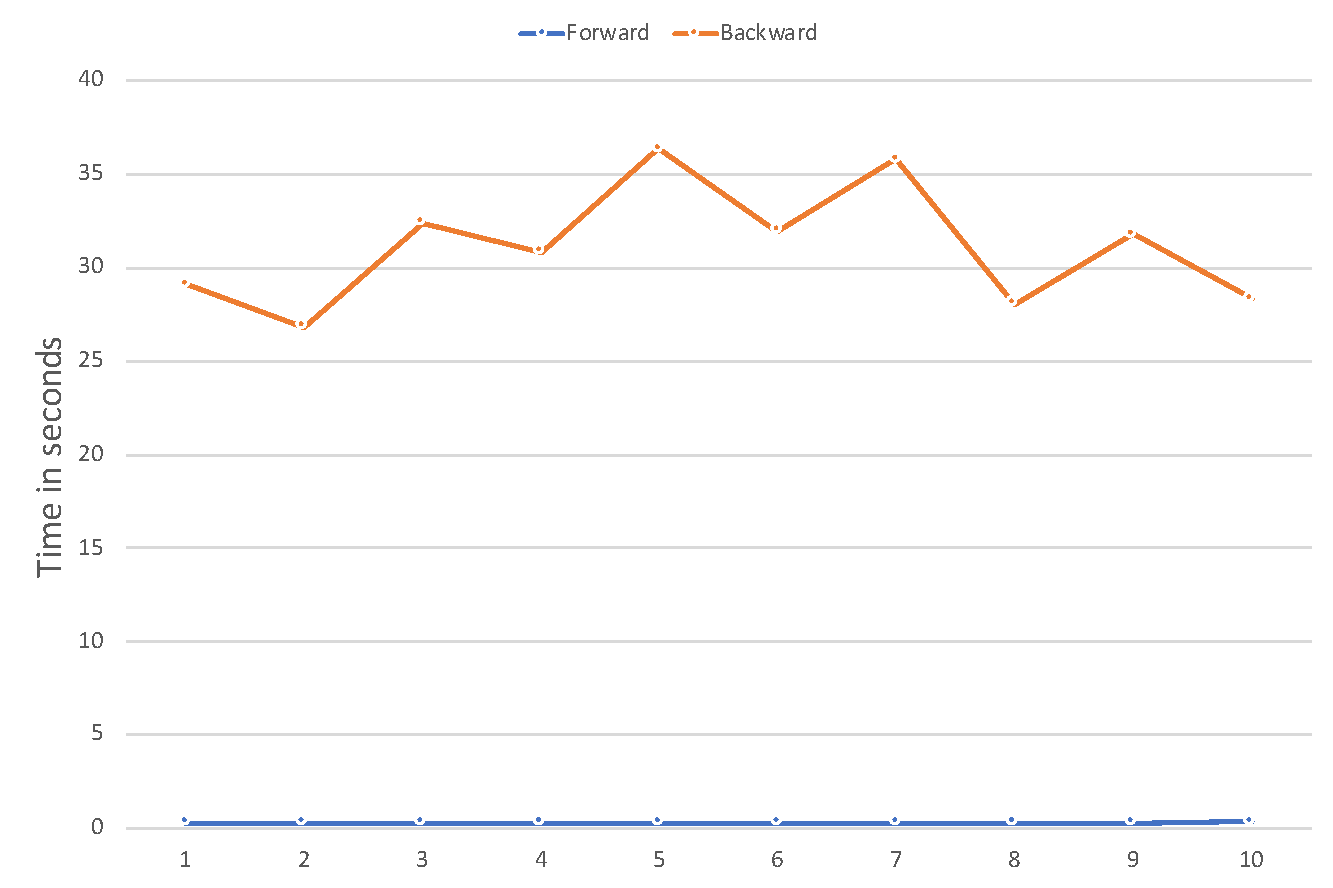
\includegraphics[width=0.8\textwidth]{./Images/seq-iter-curve.pdf}
    \caption{Multiple runs of each cases presented above}
    \label{fig:MO-seq-iter-curve}
\end{figure}

\begin{figure}[H]
    \centering
    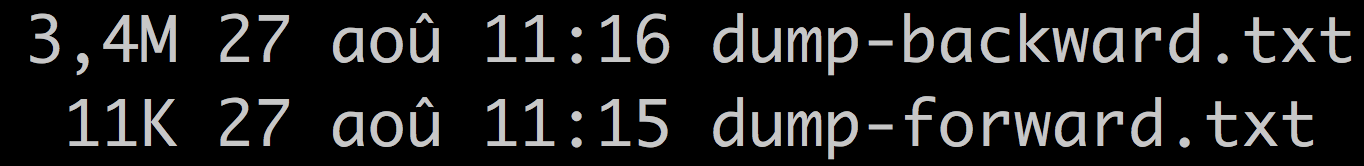
\includegraphics[width=0.6\textwidth]{./Images/dump-size}
    \caption{Screenshot of the size of the dump file for those two cases}
    \label{fig:MO-seq-iter}
\end{figure}

\begin{figure}[H]
    \centering
    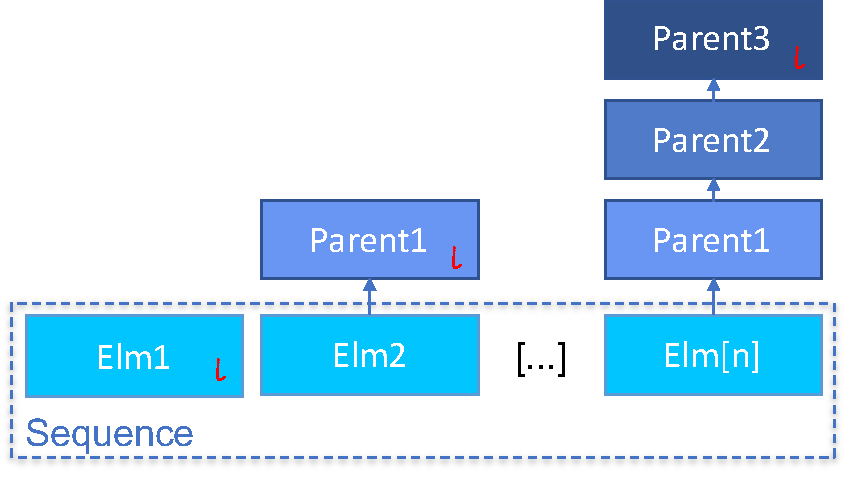
\includegraphics[width=0.8\textwidth]{./Images/seq-iter-schematic.pdf}
    \caption{Illustration of the \emph{Sequence} in this example}
    \label{fig:MO-seq-iter-schematic}
\end{figure}

%===============================================================================
% Model object alternative design
%===============================================================================

\section{Alternative design of the model object}
\label{Sec:MO-alt-design}

% separate methods from variables/data
% exploration of other type of object model
%  performance compareson / explanation
% - didn't help on average on the current use of MAD (way more data fetched than
%   functions used) but this model is kept on the side and might be reintroduce
%   depending of the evolution of the curently beta MAD application.